%\documentclass{cumcmthesis1}
\documentclass[withoutpreface,bwprint]{cumcmthesis1} %去掉封面与编号页,电子版提交的时候使用。


\usepackage[framemethod=TikZ]{mdframed}
\usepackage{url}   % 网页链接
\usepackage{subcaption} % 子标题
\title{基于仿真测试的“板凳龙”运动问题}
\tihao{A}
\baominghao{4321}
\schoolname{中山大学}
\membera{张洋 }
\memberb{邓俊辉 }
\memberc{殷润轩 }
\supervisor{ }
\yearinput{2024}
\monthinput{09}
\dayinput{22}

\begin{document}

\maketitle
\begin{abstract}
针对问题1,运用几何分析与螺线方程,可以求解龙身前把手与后把手实时位置与时间之间的关系。对于板凳的任意两点,必然满足以下两个式子,进而能够求解出问题1.\par
\[
\begin{array}{l}
\left(x_{1}-x_{2}\right)^{2} 
+\left(y_{1}-y_{2}\right)^{2} 
=L^{2}
\end{array} 
\]
\par
\[
\begin{array}{l}
(x_{1}-x_{2})* (\dot{x_{1}}-\dot{x_{2}})
+(y_{1}-y_{2})* (\dot{y_{1}}-\dot{y_{2}})
=0
\end{array}
\]
\par
我们首先通过龙头坐标与速度参数来求解第一节龙身(即龙头)的坐标与速度参数。首先用极坐标方程来表示螺旋线轨迹,根据轨迹方程与角速度的关系列出微分方程,对等式两边积分可以求出龙头把手中心的极坐标表达式,并将其转换为平面坐标表达式。\par
计算出龙头的坐标与速度参数之后,可以顺推出其余节龙身的坐标与速度参数,其约束条件分别是两点均位于螺旋线上,同时
两点直线距离为定值$L$(即上式)。由于第一节龙身被龙头牵引,因此不难判断龙身的$\theta_1$要大于龙头的$\theta_0$,假设两者的夹角为
$\Delta  \theta$ ,显然$\Delta  \theta >0$。我们让$\Delta  \theta$ 从0开始逐渐变大,直至两点的距离恰好为$L$.
根据三角余弦定理,我们通过两点的螺旋半径长度和夹角来进一步列出方程,并用MATLAB仿真得出龙头的位置结果。\par
针对问题2,根据问题2的具体要求,终止运动必然涉及板凳之间的碰撞,因此我们首先定义考虑板凳碰撞的定义,随后给出相互碰撞的约束条件。显然,需要考虑板凳的长度、宽度以及相邻板凳的连接方式。\par
根据实际情况,我们根据速度的不同大小、结合问题1所建立的模型,逐步增加时间,计算每个时刻板凳的位置,并检查其是否满足先前定义的碰撞条件。用MATLAB对其进行模拟,代码运行得出具体的数据,计算出最终的结果。
\end{abstract}

\section{问题背景与重述}
\subsection{问题背景}
本文所研究的问题基于“板凳龙”这一独特的文化活动。“板凳龙”又称“盘龙”,这是一种在浙闽地区流传已久的传统地方民俗文化活动。当地的居民将几十条乃至上百条的板凳首尾相连,形成蜿蜒曲折的“盘龙”,整体呈圆盘状。\par
本文所研究的问题正是基于这一文化活动给出的具体化数学问题。问题要求我们对一条整体为螺线结构的“盘龙”进行分析,从实际的物理现象中抽离出数学物理模型,建立方程并求解。题目给出了每条板凳的结构与相关数据。\par
\subsection{问题重述}
问题1给出了舞龙队行进时的速度、螺线的螺距、龙头的初始位置等多个条件,并要求我们解出0时刻、1分钟、2分钟、3分钟、4分钟以及5分钟时刻多个龙身前把手与后把手的速度与坐标。\par
问题2要求我们给出舞龙队行进的终止时间,使得板凳之间不发生碰撞,并给出多个龙身前把手与后把手的速度与坐标。\par
问题3提出,从盘入到盘出的全过程,舞龙队将由顺时针盘入调头切换为逆时针盘出,这需要我们给出合适的调头空间。题目中给出了圆形的调头空间,要求给出约束条件,使得龙头前把手能够沿着相应的螺线盘入到调头空间的边界。\par
问题4提出,盘出螺线与盘入螺线关于螺线中心呈中心对称,舞龙队在问题3设定的调头空间内完成调头,使得保持各部分相切的情况下调头曲线变短。\par
问题5提出,在问题4的预设框架下,保持龙头的行进速度不变,确定出各部分速度不超过2m/s基础上的龙头最大行进速度。
\section{问题分析}
\subsection{问题1的分析}
第一问要求建立模型计算舞龙队在螺线上运动时的位置和速度。这个问题主要涉及空间曲线上的运动分析。首先我们需要建立螺线弧长与角度之间的参数方程,然后根据龙头的运动速度和初始位置,推导出龙头在不同时刻的位置。接下来,从物理学的角度出发,考虑到板凳之间的连接关系,可以通过龙头的位置逐步计算出龙身和龙尾各部分的位置。速度的计算可以通过位置对时间的导数得到。\par

\par
这个问题的关键在于准确描述螺线和板凳龙的几何关系。可能使用的模型包括参数方程模型和运动学模型。在算法方面,我们使用了标准数值方法,利用物理学公式来求解运动方程。我们在MATLAB上实现了这个模型。
\subsection{问题2的分析}
第二问要求确定舞龙队盘入的终止时刻,这涉及到碰撞检测的问题。首先我们需要定义板凳之间的碰撞条件,可能需要考虑板凳的长度、宽度以及相邻板凳之间的连接方式。然后,基于问题1的模型,逐步增加时间(我们定义的步长为1s),计算每个时刻板凳的位置,并检查是否满足碰撞条件。\par
这个问题需要使用几何模型来描述板凳之间的空间关系,并结合运动学模型来分析板凳的位置变化。在算法方面,我们使用近似法与逐步逼近的方法来寻找临界时刻。同时,由于涉及到大量的碰撞检测计算,我们使用空间分割等技术提高了计算效率。
\subsection{问题3的分析}
第三问要求确定最小螺距,使龙头能够盘入到调头空间边界。这是一个优化问题,需要在满足约束条件的前提下最小化螺距。首先我们需要建立螺距与螺线曲线之间的关系模型,然后考虑龙头前把手能够到达调头空间边界的条件。\par
在这个问题中我们使用了优化模型。同时,由于螺线的特性,我们结合微分几何的知识来分析螺线的性质。在求解算法方面,我们使用了X算法来搜索理论上的最优解。此外,我们同时注意到问题的边界条件和约束条件的处理。
\section{模型假设与数学公式}
\subsection{模型假设}
问题一要求我们建立数学模型来描述舞龙队在螺线上盘入时的运动状态,包括位置和速度。这个问题涉及到空间几何和运动学的知识,需要我们深入分析板凳龙的结构特征和运动特性。首先,需要建立一个合适的坐标系统用来描述板凳龙的运动。考虑到螺线的特性,我们选择使用极坐标系。在这个坐标系中,可以方便地使用极径(r)和极角(θ)来表示板凳龙上每个点的位置。其次,我们需要仔细分析板凳龙的结构。板凳龙由223节板凳组成,包括龙头、龙身和龙尾,每节板凳的长度和宽度都是已知的。板凳之间通过把手连接。再次,我们需要考虑板凳龙的运动特性,题目给出了龙头前把手的行进速度和初始位置,这为我们建立运动方程提供了重要的边界条件。最后,我们需要考虑如何将板凳龙的运动与螺线的几何特性结合起来,螺线的螺距是已知的,这将带助我们建立螺线的参数方程。\par
基于上述思路分析,我们提出一种空间螺线运动学模型来描述板凳龙的运动,这个模型的核心思想是将板凳龙的运动分解为两个部分:切向运动和法向运动。我们首先建立螺线的参数方程,然后利用龙头前把手的运动作为基准,推导出整个板凳龙的运动方程,在这个模型中,我们将板凳龙简化为一系列连续的点,每个点代表一个把手的中心。这样的简化使我们能够更容易地处理板凳龙的运动,同时保留了问题的本质特征。\par
我们的模型考虑了以下几个关键因素:首先,螺线的几何特性,包括螺距和初始位置。其次,板凳龙的结构特征,包括每节板凳的长度和把手之间的距离。再次,龙头前把手的运动特性,包括初位置和恒定的行进速度。最后,板凳龙各部分之间的相对运动关系,即后面的板凳如何跟随前面的板凳运动。
\subsection{数学公式}
首先,我们需要建立极坐标系下螺线的参数方程,可以简单表示为下式。
\begin{equation}
\label{eq1}
    r = a*{\theta}
\end{equation}
\par
其中r代表极径,\text{$\theta$}是极角,a则是一个人为定义的常数,表示螺线覆盖区域的紧密程度。在本题要求中,a与螺距L有关,具体可以表示为
\begin{equation}
    \label{eq1}
    a  = \frac{p}{2\pi}
\end{equation}
利用板凳运动时的特征,我们画出如下示意图,并根据示意图与相应的数学关系推出关键物理量之间的关系式。
\begin{figure}
    \centering
    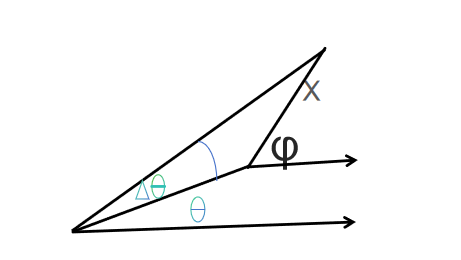
\includegraphics[width=0.5\linewidth]{CUMCMThesis-master/figures/简图.png}
    \caption{示意图}
    \label{fig:enter-label}
\end{figure}
\begin{equation}
    \frac{r(\theta_1)}{}
\end{equation}
\section{符号说明}
\begin{table}[h!]
    \centering
    \caption{符号说明三线表}
    \begin{tabular}{c|cc}
    \toprule % 顶部线
    符号 & 出现章节&含义说明 \\
    \midrule % 中间线
    $(x_{0}(t),y_{0}(t))$ & \textbf{5.2}&龙头坐标 \\
    $(L)$ &\textbf{5.2}&螺线螺距  \\
    \bottomrule % 底部线
    \end{tabular}
    \end{table}


\section{模型的建立与求解}
\subsection{\textbf{问题1}龙头位置与速度参数求解}
用极坐标方程表示的螺旋线轨迹
\[
r(\theta)=\frac{0.55 \theta}{2 \pi}
\]
\par
根据轨迹方程与角速度关系有:
\[
    r(t)=\frac{0.55 \theta(t)}{2 \pi} 
\]
\[
    \frac{v(t)}{r(t)}=-\frac{d \theta}{dt}=-\omega (t)
\]
\par
两边积分可得:
\[
\int_{32 \pi}^{\theta}  \theta (t)\,dt =-\frac{2 \pi}{55}\int_{0}^{t}  \,dt 
\]

求得龙头把手中心极坐标表达式:
\begin{align*}
    \begin{cases}
        \theta(t)=\sqrt{(32\pi)^2-\frac{80}{11}\pi t}\\
        r(t)=\frac{0.55 \theta(t)}{2 \pi} 
    \end{cases}
\end{align*}
\par
相应地可以转换成平面坐标表达式
\begin{align*}
    \begin{cases}
        x(t) = r(t) \cos \theta(t)\\
        y(t) = r(t) \sin \theta(t)\\
    \end{cases}
\end{align*}
\par
为了求出当前时刻的横纵方向分速度$v_{0x}$和$v_{0y}$,可以通过链式法则对上面的式子进行求导:
\begin{align*}
    \begin{cases}
        v_{0x}(t) = \cos\theta(t) \cdot \frac{dr(t)}{dt} - r(t) \sin\theta(t) \cdot \frac{d\theta(t)}{dt} \\
        v_{0y}(t)= \sin\theta(t) \cdot \frac{dr(t)}{dt} + r(t) \cos\theta(t) \cdot \frac{d\theta(t)}{dt}
    \end{cases}
\end{align*}
\par
其中:
\begin{align*}
    \begin{cases}
        \frac{dr(t)}{dt} = -\frac{1}{\sqrt{(32\pi)^2 - \frac{80}{11}\pi t}}\\
        \frac{d\theta(t)}{dt} = -\frac{0.4\pi}{11 \sqrt{(32\pi)^2 - \frac{80}{11}\pi t}}
    \end{cases}
\end{align*}
\subsection{\textbf{问题1}其他各节龙身位置与速度参数求解}
我们首先通过龙头坐标与速度参数来求解第一节龙身的坐标与速度参数,其约束条件分别是两点均位于螺旋线上,同时
两点直线距离为定值$L$。由于第一节龙身被龙头牵引,因此不难判断龙身的$\theta_1$要大于龙头的$\theta_0$,假设两者的夹角为
$\Delta  \theta$ ,显然$\Delta  \theta >0$。我们让$\Delta  \theta$ 从0开始逐渐变大,直至两点的距离恰好为$L$.
根据三角余弦定理,我们通过两点的螺旋半径长度和夹角来列出方程:
\begin{align*}
    \begin{cases}
        L^2=r(\theta_1)^2+r(\theta_1+\Delta  \theta)^2-2r(\theta_1)r(\theta_1+\Delta  \theta) \cos \Delta \theta\\
        r(\theta)=0.55 \theta /2 \pi 
    \end{cases}
\end{align*}
\par
不难发现,这个方程属于超越方程,只能通过牛顿-拉夫森法等方法不断优化以求得一个精度较高的数值解(大约小数点后6位)。\par
然而反复迭代的方法非常耗时,因此我们采取了近似的方法,将螺线等分成数段,并将其近似看成多个小段的、半径不同的圆弧,再利用弧长公式计算出各节龙身的位置与速度(方法如下图)。我们所取的最小步长为1s,此时能够得到最为精确的结果。\par
经过不断迭代与优化,我们得出了相对精确的位置结果,保留小数点后五位数字。

\begin{table}[h!]
    \caption{位置结果}
    \centering
    \begin{tabular}{|c|c|c|c|c|c|c|}
    \hline
     & $0s$ & $60s$ & $120s$ & $180s$ & $240s$ & $300s$ \\
    \hline
    龙头 x (m) &8.8&5.796934&-4.090654&-2.953259&2.578971&4.431365 \\
    \hline
    龙头 y (m) & 0.000000 & -5.773329 & -6.300643 & 6.099638 &-5.363954&2.298233 \\
    \hline
     第1节龙身x& 8.366286&3.456016 & -6.111764 &-0.194664 & -191234  & 4.919684 \\
    \hline
     第1节龙身y& 2.819001 & -7.381867 &-4.310255  & 6.737217 & -5.906572&-0.466255  \\
    \hline
     第51节龙身x& -9.512018 & 5.486829 & -1.43511 & 3.932879 & 0.397575 & 0.227612 \\
    \hline
     第51节龙身y& 1.385148&4.680284& 6.28097   & 3.942671 & 4.512326 & -3.160608 \\
    \hline
     第101节龙身x& 2.841064 & 3.68234 & -5.07733 & -3.454 & -2.47359 & 0.555436 \\
    \hline
     第101节龙身y& -9.938777& 4.902125 & 1.148161& 2.164192 & 0.20858 & 0.125698 \\
    \hline
     第151节龙身x& 10.877538& 0.124579 & -3.54136 & 0.133836 & -1.65013 & 2.255574 \\
    \hline
     第151节龙身y& 1.727014& -4.81315 & 0.409225 & -1.51431 & 0.002419& 10.325175 \\
    \hline
     第201节龙身x& 4.671434 & -2.35762 & 4.940488 & 0.532093 & -1.24801 & 8.958199 \\
    \hline
     第201节龙身y& 10.67392 & 1.802727 & 0.406542 & 0.73535 & 1.916431 & -4.124826 \\
    \hline
     龙尾(后)x& -5.427245 & 1.281067 & -0.406418 & 1.741699 & 0.019065 & -4.909683 \\
    \hline
     龙尾(后)y& -10.61406 & -0.94886 & -4.25146 & 0.734097 & 0.147523 & 8.173638 \\
    \hline
    \end{tabular}
    \label{tab:example}
    \end{table}

\begin{table}[h!]
    \caption{速度结果}
    \centering
    \begin{tabular}{|c|c|c|c|c|c|c|}
    \hline
     & $0s$ & $60s$ & $120s$ & $180s$ & $240s$ & $300s$ \\
    \hline
    龙头 & 1.00005& 1.00006&1.00007&1.00008&1.00011&1.00015\\
    \hline
     第1节龙身& 1.00004 & 1.00004 & 1.00007 & 1.00005& 1.00006 & 1.00005 \\
    \hline
     第51节龙身& 0.99989 & 0.99984 & 1.00005 & 0.99966 &0.99945 & 0.99896 \\
    \hline
     第101节龙身& 0.99977 & 0.9997 & 0.99978 & 0.99942 & 0.99911 & 0.99845 \\
    \hline
     第151节龙身& 0.99969 &0.9996  &0.9996  & 0.99926 & 0.99889& 0.99816 \\
    \hline
     第201节龙身& 0.9996 & 0.99952 & 0.99947 & 0.99914 & 0.99875 & 0.99796 \\
    \hline
     龙尾(后)& 0.99949 & 0.99949 & 0.99934 & 0.9991 & 0.9987 & 0.9979\\
    \hline
    \end{tabular}
    \label{tab:example}
    \end{table}









\begin{appendices}

\section{\textbf{问题1}}


\begin{lstlisting}[language=matlab]
   clc, clear;
time_total = 300; % 总时间 300秒
dt = 1; % 时间步长 1秒
dt_small = 0.0001; % 用于计算速度的小时间步长
n_sections = 224; % 把手数量

% 时间数组
time_steps = 0:dt:time_total;

% 初始化存储位置的矩阵
positions = zeros(n_sections * 2, length(time_steps)); 
velocity = zeros(n_sections, length(time_steps)); % 因为速度在相邻的整数秒之间计算

% 定义一个函数,输入时间t,返回t时刻的所有把手位置
function positions = calculate_positions_at_time(t)
    % 设定参数
    n_sections = 224; % 把手数量
    pitch = 0.55; % 螺距55cm
    % 板凳长度
    distance_1 = 2.86; %龙头两个把手的距离
    distance_2 = 1.65; %龙身两个把手的距离
    theta_initial = 2 * pi * 16; % 第16圈起始角度
    % 初始化存储位置的矩阵
    positions = zeros(n_sections * 2, 1);
    
    % 计算当前时刻的龙头角度和半径
    theta = sqrt(theta_initial^2 - 4 * pi / pitch * t); % 当前时刻的角度变化
    radius = pitch * theta / (2 * pi); % 螺线半径
    
    % 计算龙头的位置
    x_head = radius * cos(theta); % x 位置
    y_head = radius * sin(theta); % y 位置
    
    % 将龙头位置保存到矩阵(第1行和第2行分别为x和y)
    positions(1) = x_head;
    positions(2) = y_head;
    
    % 计算每一节龙身的位置
    for i = 2:n_sections
        %两个把手之间的距离
        if (i == 2)
            distance = distance_1;
        else
            distance = distance_2;
        end
        delta_theta = distance / radius;
        theta = theta + delta_theta;
        radius = 0.55 * theta / (2 * pi);
        % 计算该节板凳的 x 和 y 坐标
        x_i = radius * cos(theta);
        y_i = radius * sin(theta);
        
        % 保存该节板凳的位置 (注意行号是 2i-1 和 2i)
        positions(2*i-1) = x_i;
        positions(2*i) = y_i;
    end
end

% 计算每秒钟的位置信息
for t_idx = 1:length(time_steps)
    t = time_steps(t_idx);
    positions(:, t_idx) = calculate_positions_at_time(t);
end

% 计算整数秒之间的速度,使用 t 和 t+0.0001 之间的位移来计算
for t_idx = 1:length(time_steps)
    % 当前时刻 t_now 和 t+0.001 秒时刻
    t_now = time_steps(t_idx);
    t_small = t_now + dt_small;
    
    % 获取所有把手在 t_now 时刻的位置
    pos_now = calculate_positions_at_time(t_now);  % 返回一个 2*n_sections 大小的向量
    
    % 获取所有把手在 t+0.001s 时刻的位置
    pos_next = calculate_positions_at_time(t_small);  % 返回一个 2*n_sections 大小的向量
    
    % 将 pos_now 和 pos_next 重新分为 x, y 坐标
    x_now = pos_now(1:2:end);   % 当前时刻所有把手的 x 坐标
    y_now = pos_now(2:2:end);   % 当前时刻所有把手的 y 坐标
    x_next = pos_next(1:2:end); % t+0.001s 时刻所有把手的 x 坐标
    y_next = pos_next(2:2:end); % t+0.001s 时刻所有把手的 y 坐标
    
    % 计算速度 (vx, vy),然后计算总速度
    v_x = (x_next - x_now) / dt_small;
    v_y = (y_next - y_now) / dt_small;
    
    % 计算每个把手的速度并存储
    velocity(:, t_idx) = sqrt(v_x.^2 + v_y.^2);
end


%将结果保留六位小数
positions = round(positions, 6);
velocity = round(velocity, 6);

% 构建第一页行头,表示每节板凳的 x(m) 和 y(m) 坐标
headers_rows_1 = {'', '龙头x(m)', '龙头y(m)'};
for i = 1:n_sections-3
    headers_rows_1 = [headers_rows_1, {['第' num2str(i) '节龙身x(m)'], ['第' num2str(i) '节龙身y(m)']}];
end
headers_rows_1 = [headers_rows_1, {'龙尾x(m)', '龙尾y(m)'}];
headers_rows_1 = [headers_rows_1, {'龙尾(后)x(m)', '龙尾(后)y(m)'}];

% 构建第一页列头,表示每个时间点 (0s, 1s, 2s, ...)
headers_columns_1 = arrayfun(@(x) [num2str(x) 's'], time_steps, 'UniformOutput', false);

% 将 headers_rows_1 和 headers_columns_1 拼接到数据中
final_data_1 = [headers_rows_1', [headers_columns_1; num2cell(positions)]];

% 构建第二页行头
headers_rows_2 = {'', '龙头(m/s)'};
for i = 1:n_sections-3
    headers_rows_2 = [headers_rows_2, {['第' num2str(i) '节龙身(m/s)']}];
end
headers_rows_2 = [headers_rows_2, {'龙尾(m/s)'}];
headers_rows_2 = [headers_rows_2, {'龙尾(后)(m/s)'}];

% 构建第二页列头,表示每个时间点 (1s, 2s, 3s, ...)
headers_columns_2 = arrayfun(@(x) [num2str(x) 's'], time_steps(1:end), 'UniformOutput', false);

% 将 headers_rows_2 和 headers_columns_2 拼接到数据中
final_data_2 = [headers_rows_2', [headers_columns_2; num2cell(velocity)]];

% 保存到Excel文件,位置数据到第一页,速度数据到第二页
writecell(final_data_1, 'result1.xlsx', 'Sheet', '位置');
writecell(final_data_2, 'result1.xlsx', 'Sheet', '速度');

end
 \end{lstlisting}

\section{\textbf{问题2}}
\begin{lstlisting}[language=matlab]
clc; clear;
start_time = 0; %开始时间
dt = 0.001; % 默认时间步长
end_time = 440;%结束时间
dt_small = 0.000001; % 用于计算速度的小时间步长
n_sections = 224; % 把手数量
length_head = 3.41; % 龙头长度
length_body = 2.0;  % 龙身长度
width = 0.3; % 板凳宽度30cm
offset = 0.275; % 把手到边界的距离为 0.275m
collision_time = -1; % 初始化碰撞时间

% 时间数组
time_steps = start_time:dt:end_time;

% 定义函数计算每时刻所有把手位置
function positions = calculate_positions_at_time(t)
    n_sections = 224;
    pitch = 0.55; % 螺距55cm
    distance_1 = 2.86; %龙头两个把手的距离
    distance_2 = 1.65; %龙身两个把手的距离
    theta_initial = 2 * pi * 16; % 初始角度
    positions = zeros(n_sections * 2, 1);
    
    theta = sqrt(theta_initial^2 - 4 * pi / pitch * t); % 当前角度
    radius = pitch * theta / (2 * pi); % 螺旋半径
    
    x_head = radius * cos(theta); 
    y_head = radius * sin(theta);
    positions(1) = x_head;
    positions(2) = y_head;
    
    for i = 2:n_sections
        if (i == 2)
            distance = distance_1;
        else
            distance = distance_2;
        end
        delta_theta = distance / radius;
        theta = theta + delta_theta;
        radius = 0.55 * theta / (2 * pi);
        x_i = radius * cos(theta);
        y_i = radius * sin(theta);
        positions(2*i-1) = x_i;
        positions(2*i) = y_i;
    end
end

% 定义辅助函数,检查点是否在矩形内
function inside = is_point_in_rectangle(px, py, rect)
    x1 = rect(1,1); y1 = rect(1,2);
    x2 = rect(2,1); y2 = rect(2,2);
    x3 = rect(3,1); y3 = rect(3,2);
    x4 = rect(4,1); y4 = rect(4,2);
    
    % 使用向量叉积判断点是否在矩形内
    v1 = [x2 - x1, y2 - y1]; % 向量 v1
    v2 = [x3 - x2, y3 - y2]; % 向量 v2
    v3 = [x4 - x3, y4 - y3]; % 向量 v3
    v4 = [x1 - x4, y1 - y4]; % 向量 v4
    
    % 点相对于每条边的叉积
    cp1 = (px - x1)*(y2 - y1) - (py - y1)*(x2 - x1); % 点在边1左侧
    cp2 = (px - x2)*(y3 - y2) - (py - y2)*(x3 - x2); % 点在边2左侧
    cp3 = (px - x3)*(y4 - y3) - (py - y3)*(x4 - x3); % 点在边3左侧
    cp4 = (px - x4)*(y1 - y4) - (py - y4)*(x1 - x4); % 点在边4左侧
    
    % 如果所有叉积都为正或都为负,则点在矩形内
    inside = (cp1 >= 0 && cp2 >= 0 && cp3 >= 0 && cp4 >= 0) || ...
             (cp1 <= 0 && cp2 <= 0 && cp3 <= 0 && cp4 <= 0);
end

% 主循环,只检测龙头的碰撞
for t_idx = 1:length(time_steps)
    t = time_steps(t_idx);
    positions_now = calculate_positions_at_time(t);
    % 检查螺旋中心,当 theta 接近 0 时,停止计算
    theta_2 = (2 * pi * 16)^2 - 4 * pi / 0.55 * t;
    if theta_2 < 0
        disp(['龙头在 t = ', num2str(t), ' 秒到达螺旋中心,无法继续旋入']);
        collision_time = t;
        break;
    end
    
    % 计算龙头的两个前角,基于前后把手的位置
    x_head_front = positions_now(1);   % 龙头前把手的 x 坐标
    y_head_front = positions_now(2);   % 龙头前把手的 y 坐标
    x_head_back = positions_now(3);    % 龙头后把手的 x 坐标
    y_head_back = positions_now(4);    % 龙头后把手的 y 坐标
    
    % 计算龙头的方向向量
    dx_head = x_head_front - x_head_back;
    dy_head = y_head_front - y_head_back;
    length_vector_head = sqrt(dx_head^2 + dy_head^2);
    
    % 归一化方向向量 (使其长度为1)
    direction_x_head = dx_head / length_vector_head;
    direction_y_head = dy_head / length_vector_head;
    
    % 垂直方向向量 (用于计算龙头的左右两侧)
    perpendicular_x_head = -direction_y_head;
    perpendicular_y_head = direction_x_head;
    
    % 计算龙头的前左和前右角坐标,考虑宽度和偏移量
    x_head_front_left = x_head_front + (width / 2) * perpendicular_x_head + offset * direction_x_head;
    y_head_front_left = y_head_front + (width / 2) * perpendicular_y_head + offset * direction_y_head;
    
    x_head_front_right = x_head_front - (width / 2) * perpendicular_x_head + offset * direction_x_head;
    y_head_front_right = y_head_front - (width / 2) * perpendicular_y_head + offset * direction_y_head;
    
    % 遍历之后的所有板凳,检查是否发生碰撞
    for i = 3:n_sections
        % 当前节的后把手和前把手的位置
        x_back = positions_now(2*i-1); % 后把手
        y_back = positions_now(2*i);   % 后把手
        x_front = positions_now(2*(i-1)-1); % 前把手
        y_front = positions_now(2*(i-1));   % 前把手
        
        % 计算板凳的方向向量 (dx, dy)
        dx = x_back - x_front; % 计算前把手到后把手的向量
        dy = y_back - y_front;
        length_vector = sqrt(dx^2 + dy^2);
        
        % 归一化方向向量 (使其长度为1)
        direction_x = dx / length_vector;
        direction_y = dy / length_vector;
        
        % 垂直方向向量 (用于计算板凳的左右两侧)
        perpendicular_x = -direction_y;
        perpendicular_y = direction_x;
        
        % 计算板凳的四个角,考虑偏移量 offset 和宽度 width
        % 后右角
        x_back_left = x_back + (width / 2) * perpendicular_x + offset * direction_x;
        y_back_left = y_back + (width / 2) * perpendicular_y + offset * direction_y;
        
        % 后左角
        x_back_right = x_back - (width / 2) * perpendicular_x + offset * direction_x;
        y_back_right = y_back - (width / 2) * perpendicular_y + offset * direction_y;
        
        % 前右角
        x_front_left = x_front + (width / 2) * perpendicular_x - offset * direction_x;
        y_front_left = y_front + (width / 2) * perpendicular_y - offset * direction_y;
        
        % 前左角
        x_front_right = x_front - (width / 2) * perpendicular_x - offset * direction_x;
        y_front_right = y_front - (width / 2) * perpendicular_y - offset * direction_y;
        
        % 将这四个角点存储为矩形
        rect = [x_back_left, y_back_left;
                x_back_right, y_back_right;
                x_front_right, y_front_right;
                x_front_left, y_front_left];
        
        % 检查龙头前左、前右是否进入该矩形内
        if is_point_in_rectangle(x_head_front_left, y_head_front_left, rect) || ...
           is_point_in_rectangle(x_head_front_right, y_head_front_right, rect)
            collision_time = t;
            disp(['碰撞发生在 t = ', num2str(collision_time), ' 秒']);
            break;
        end
    end
    if collision_time > 0
        break;
    end
end

% 在碰撞时刻之前的时刻和下一个时刻计算速度
if collision_time > 0
    t_previous = collision_time - dt;
    
    % 计算碰撞前一时刻的位置
    positions_previous = calculate_positions_at_time(t_previous);
    
    % 计算下一小段的位置
    positions_next = calculate_positions_at_time(t_previous + dt_small);
    
    % 初始化存储位置和速度的矩阵 (224行, 3列)
    result_matrix = zeros(n_sections, 3);
    
    % 逐节计算每个把手的x, y和速度
    for i = 1:n_sections
        % 获取前一时刻的 x 和 y 坐标
        x_previous = positions_previous(2*i-1);
        y_previous = positions_previous(2*i);
        
        % 获取碰撞时刻的 x 和 y 坐标
        x_collision = positions_next(2*i-1);
        y_collision = positions_next(2*i);
        
        % 计算速度 (基于前后两个时刻的位移)
        v_x = (x_collision - x_previous) / dt_small;
        v_y = (y_collision - y_previous) / dt_small;
        velocity_i = sqrt(v_x^2 + v_y^2); % 计算总速度
        
        % 将结果存储到矩阵中
        result_matrix(i, 1) = x_previous;   % x 坐标
        result_matrix(i, 2) = y_previous;   % y 坐标
        result_matrix(i, 3) = velocity_i;   % 速度
    end

    % 构建行头
    headers_rows = {'', '龙头'};
    for i = 1:n_sections-3
        headers_rows = [headers_rows, {['第' num2str(i) '节龙身']}];
    end
    headers_rows = [headers_rows, {'龙尾'}];
    headers_rows = [headers_rows, {'龙尾(后)'}];

    % 构建列头,表示x,y和速度
    headers_columns = {'横坐标x(m)','纵坐标y(m)','速度(m/s)'};

    % 将 headers_rows 和 headers_columns 拼接到数据中
    final_data = [headers_rows', [headers_columns; num2cell(result_matrix)]];

    % 保存到Excel文件
    writecell(final_data, 'result2.xlsx');
end




\end{lstlisting}


 
\end{appendices}

\end{document} 